% THIS IS SIGPROC-SP.TEX - VERSION 3.1
% WORKS WITH V3.2SP OF ACM_PROC_ARTICLE-SP.CLS
% APRIL 2009
%
% It is an example file showing how to use the 'acm_proc_article-sp.cls' V3.2SP
% LaTeX2e document class file for Conference Proceedings submissions.
% ----------------------------------------------------------------------------------------------------------------
% This .tex file (and associated .cls V3.2SP) *DOES NOT* produce:
%       1) The Permission Statement
%       2) The Conference (location) Info information
%       3) The Copyright Line with ACM data
%       4) Page numbering
% ---------------------------------------------------------------------------------------------------------------
% It is an example which *does* use the .bib file (from which the .bbl file
% is produced).
% REMEMBER HOWEVER: After having produced the .bbl file,
% and prior to final submission,
% you need to 'insert'  your .bbl file into your source .tex file so as to provide
% ONE 'self-contained' source file.
%
% Questions regarding SIGS should be sent to
% Adrienne Griscti ---> griscti@acm.org
%
% Questions/suggestions regarding the guidelines, .tex and .cls files, etc. to
% Gerald Murray ---> murray@hq.acm.org
%
% For tracking purposes - this is V3.1SP - APRIL 2009

\documentclass{acm_proc_article-sp}

\usepackage{graphicx}
\usepackage{epsfig}
%% The amssymb package provides various useful mathematical symbols
\usepackage{amssymb}
\usepackage{amsmath}
\usepackage{algorithm}
\usepackage[noend]{algpseudocode}
\usepackage{float}

\begin{document}

\title{Predicting Adverse Thermal Events in a Smart Building\thanks{Team 2, Project C3, Host: Rodney Martin}}

%
% You need the command \numberofauthors to handle the 'placement
% and alignment' of the authors beneath the title.
%
% For aesthetic reasons, we recommend 'three authors at a time'
% i.e. three 'name/affiliation blocks' be placed beneath the title.
%
% NOTE: You are NOT restricted in how many 'rows' of
% "name/affiliations" may appear. We just ask that you restrict
% the number of 'columns' to three.
%
% Because of the available 'opening page real-estate'
% we ask you to refrain from putting more than six authors
% (two rows with three columns) beneath the article title.
% More than six makes the first-page appear very cluttered indeed.
%
% Use the \alignauthor commands to handle the names
% and affiliations for an 'aesthetic maximum' of six authors.
% Add names, affiliations, addresses for
% the seventh etc. author(s) as the argument for the
% \additionalauthors command.
% These 'additional authors' will be output/set for you
% without further effort on your part as the last section in
% the body of your article BEFORE References or any Appendices.

\numberofauthors{4} %  in this sample file, there are a *total*
% of EIGHT authors. SIX appear on the 'first-page' (for formatting
% reasons) and the remaining two appear in the \additionalauthors section.
%
\author{
% You can go ahead and credit any number of authors here,
% e.g. one 'row of three' or two rows (consisting of one row of three
% and a second row of one, two or three).
%
% The command \alignauthor (no curly braces needed) should
% precede each author name, affiliation/snail-mail address and
% e-mail address. Additionally, tag each line of
% affiliation/address with \affaddr, and tag the
% e-mail address with \email.
%
% 1st. author
\alignauthor
Jenna MacCarley\\
	   \affaddr{Carnegie Mellon University}\\
       \email{jmaccarl@andrew.cmu.edu}
% 2nd. author
\alignauthor
Federico Ponte\\
       \affaddr{Carnegie Mellon University}\\
       \email{federico.ponte@sv.cmu.edu}
% 3rd. author
\alignauthor Victor Hu\\
       \affaddr{Carnegie Mellon University}\\
       \email{vyh@andrew.cmu.edu}
\and  % use '\and' if you need 'another row' of author names
% 4th. author
\alignauthor Diane Yang\\
       \affaddr{Carnegie Mellon University}\\
       \email{dan.yang@sv.cmu.edu}
}
% There's nothing stopping you putting the seventh, eighth, etc.
% author on the opening page (as the 'third row') but we ask,
% for aesthetic reasons that you place these 'additional authors'
% in the \additional authors block, viz.

% Just remember to make sure that the TOTAL number of authors
% is the number that will appear on the first page PLUS the
% number that will appear in the \additionalauthors section.

\maketitle
\begin{abstract}
The purpose of this research is to use machine learning methods to create an effective anomaly detection system, designed to predict real adverse thermal events in a smart building located on NASA's Sustainability Base. Our project centers around the design of an effective anomaly detection system modeled after ACCEPT, a state of the art system built by NASA engineers for comparing various regression models and detection methods. Our goal was to create a similarly performing system, but use open-source Python libraries as opposed to proprietary software based on MATLAB. Ultimately, we were able to create a highly effective system that could predict a cold event's occurrence using the given data with a 0.6\% False Positive rate and a 3.1\% Missed Detection rate. We compared our research results to those from another student team from Cornell, that used ACCEPT to predict cold events with the same data, and found that our system design results rivaled theirs. The source code for our research is publicly available online\footnote{https://github.com/fedep3/sdl}.
\end{abstract}

\section{Introduction \textit{(Jenna)}}
NASAs Sustainability Base \cite{nasasb} is a green building located in the Ames Research Center at Moffet Field, CA and among the greenest in the federal government. It is LEED platinum certified, achieving the highest rating for sustainability through its innovative design of architecture, resource recycling systems, renewable power generation and advanced sensing systems. The advanced sensing systems in the building are advertised as ``anticipating and reacting to changes in sunlight, temperature, wind, and occupancy and will be able to optimize its performance automatically, in real time, in response to internal and external changes`` \cite{nasasb}. However, despite these advancements in technology there have been numerous complaints that rooms in the building are too cold. Since the building incorporates thousands of sensors, including 2636 thermal sensors specifically \cite{Cornell}, it is difficult to narrow down where this issue of cold complaints may be coming from. 

Our goal for this research is to use machine learning models to understand what events may be triggering an abnormally cold temperature in the building and be able to predict instances of it. Our research is based off of a project out of Cornell university, which had the same goal of predicting adverse thermal events in this building \cite{Cornell}. These researchers used ACCEPT (Adverse Condition and Critical Event Prediction Toolbox), a MATLAB framework developed by NASA which is designed to compare and contrast the performance of various machines learning algorithms and anomaly detection mechanisms \cite{accept}. Our goal for this project is to expand upon their research, but develop our own framework in Python using existing machine learning libraries such as scikit-learn \cite{scikitlearn} and Pyflux \cite{pyflux}. Our goal was to ultimately replicate and improve upon the results from the Cornell researchers, creating higher accuracy in the prediction of the anomalous cold events determined by the resulting false positive and missed detection rates using the same data.

This paper is organized as follows: First we will discuss the background of the project, including research on anomaly detection methods such as those used in NASA's ACCEPT framework. We will then discuss the design of our system, beginning with our regression toolbox which implements a comparison of different regression algorithms, to our detection toolbox which implements a comparison of different detection methods. Next, we will present our results, demonstrating sufficient success in building an effective mechanism for detecting anomalous cold events. Finally, we will conclude and discuss future work for improving our system.

\section{Background\textit{(Diane/Jenna)}} 
Predicting adverse thermal events in this smart building lies in the model of anomaly detection since cold events occur as anomalies. There are a variety of methods which can be used to address the problem. First, we will discuss basic ideas relating to anomaly detection and then introduce NASA's ACCEPT framework, which our system design is based off of. We will also discuss the related research from Cornell university which provides a good comparison for our work.

\subsection{Anomaly Detection\textit{(Diane)}}
The general architecture of all anomaly detection methods consists of the following basic three modules or stages: parameterization, training and detection (see Figure \ref{fig:anomaly}).

\textbf{Parameterization} aims at collecting raw data from a monitored environment. The raw data should be representative of the system to be modeled, (e.g. Packet data from a network).

\textbf{The training stage} seeks to model the system using manual or automatic methods. The behaviors represented in the model will differ accordingly with the technique used.

\textbf{Detection} compares the system generated results in the training stage with the selected parameterized data portion. Threshold criteria will be selected to determine anomalous data events\cite{Anomalyd}. 

\begin{figure}
\centering
\centering
    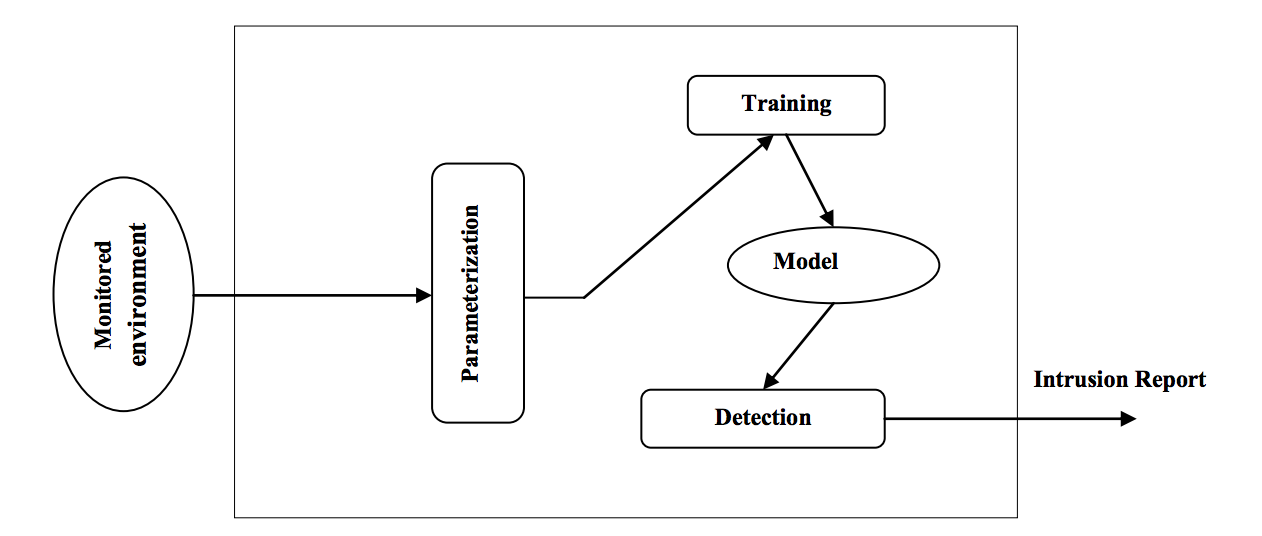
\includegraphics[scale=0.4]{figures/11.png}
\caption{Generic Anomaly Detection Functional Architecture}
\label{fig:anomaly}
\end{figure}

\subsubsection{Anomaly Detection Techniques}
There are three types of anomaly views.
Supervised view: anomalies are what some user labels as anomalies. The data comprises of fully labeled training and test datasets. An ordinary classifier can be trained first and applied afterwards. The most common supervised algorithms are,
Supervised Neural Networks, Support Vector Machines(SVM), k-Nearest Neighbors, Bayesian Networks and Decision Tree \cite{decisiontree}.

Unsupervised view: anomalies are outliers (points of low probability) in the data.  The idea is evaluating the data solely based on intrinsic properties of the dataset. Furthermore, there is also no distinction between a training and a test dataset. Typically, distances or densities can be used to give an estimation what is normal and what is an outlier\cite{Anomalystep}. 

Semi-supervised view: in this situation, the training data only consists of normal data without any anomalies. The basic idea is that a model of the normal class is learned and anomalies can be detected afterwards by deviating from that model. Of course, in general any density estimation method can be used to model the probability density function of the normal classes, such as Gaussian Mixture Models\cite{GaussianM} or Kernel Density Estimation\cite{KernelD}.

% swapped out 'this article' for 'our research'
Our research only focuses on semi-supervised anomaly detection setup. And ACCEPT, which our system is modeled after, is based on the Multivariate State Estimation Technique(MSET).
\newpage

\subsubsection{Multivariate State Estimation Technique}
MSET\cite{MSET} is a nonlinear, nonparametric modeling
method that was originally developed by Argonne National
Laboratory (ANL) for high-sensitivity proactive fault monitoring applications in commercial nuclear power applications. The MSET software described is configured to detect instrument degradation and perform system diagnostics with higher accuracy and faster response time than prior art techniques. 

The implementation of this technique requires a few steps shown as follows:

\textbf{Training step:} A training procedure is developed to characterize the monitored equipment and build a model. There are some characteristics about Training Data: a) Containing all modes and ranges of operation b) Not containing any operating anomalies. 
After a comprehensive and error-free set of training data has been assembled, the MSET training algorithms are used to build an MSET model of the asset. The training procedure evaluates the training data and selects a subset of the training data observations (training vectors)that are determined to best characterize the asset's normal operation. 

\textbf{Monitoring step:} This step uses the previously trained MSET model to estimate the expected values of the signals via newly acquired observations. 
A weighting method is used to produce the estimate by combining the example data values. Those examples most similar to the current observation are heavily weighted while those that are dissimilar are negligibly weighted. Similarity between the current observation and the learned examples is computed using sophisticated multivariable pattern matching techniques. The weighted combination of the most similar learned examples is used to compute the estimated signal values given the current observed signal values. 
After prediction, residuals can be obtained through computing the difference between a signal's predicted value and its directly sensed value. 
The MSET technique provides an extremely accurate estimate of sensor signals, with error rates that are typically 1\% to 2\% of the standard deviation of the input signal, which is excellent.

\textbf{Fault detection step:} This step uses Sequential Probability Ratio Test (SPRT) technique to determine whether the residual error value is uncharacteristic of the learned process model and thereby indicative of a sensor or equipment fault. For sudden, gross failures of a sensor or a subsystem, this procedure enunciates the disturbance as fast as a conventional threshold limit check.
In operation, a time series of residual values are evaluated to determine whether the series of values is characteristic of the expected distribution or alternatively of some other specified distribution. Four possible fault-type distributions are considered in the current software. These are: 1) the residual mean value has shifted high; 2) the residual mean value has shifted low; 3) the residual variance value has increased; and 4) the residual variance value has decreased. 

NASA's ACCEPT framework that our research based on is developed according to MSET model. They share some similarities and have differences. 

\subsection{ACCEPT Framework \textit{(Jenna)}}
ACCEPT stands for Adverse Condition and Critical Event Prediction Toolbox, and is an architectural  framework developed by NASA for predicting anomalous events in real-time processes \cite{accept}. It is designed to utilize and compare a variety of machine learning techniques in order to provide a performance assessment of results for various applications. It is modeled after MSET (Multivariate State Estimation Technique), which is a state of the art statistical modeling technique originally developed by Argonne National Laboratory for online nuclear power plant monitoring \cite{MSET}. MSET and ACCEPT share a similar fundamental basis: creating an accurate model of an asset from a sample of its normal operating data, and comparing the output from that model to the actual observation. Deviations detected from the model are used to predict process anomalies. MSET and ACCEPT differ, however, in that ACCEPT uses a variety of machine learning techniques to parameterize the underlying models rather than the more restrictive set used by MSET. Therefore, ACCEPT is a flexible system and an ideal model to observe for the problem we are exploring in this paper, where cold events are a rare occurrence.

\subsubsection{Architecture}
ACCEPT architecture (see Figure \ref{fig:accept-arch}) is divided into Regression and Detection steps, with two distinct goals of finding the best-fitting regression model, then using the resulting predictions to configure the detection system and generate alarm statistics. All data is preprocessed and filtered using z-score normalization and feature selection. The training data, or the optimal data used that does not contain anomalous events, is provided to the regression toolbox to compare various static regression models to best fit the optimal system operation. Autoregressive models are not currently implemented in the architecture. All data, including the training data, validation data and testing data (only the first not containing anomalous events), is provided to the detection toolbox to configure the alarm system. The detection toolbox receives the residual prediction values given by \[r_t = \mid y_{t,pred} - y_{t,actual} \mid\] which represent the absolute difference between the regression algorithm output and the actual value of the output at a time t. These are generated over time and used to create various alarm statistics, with an Optimal Alarm System, Predictive Alarm System, SPRT Hypotheses and Redline Alarm System mechanisms implemented. The output from this system will be a binary classification indicating that an anomalous event will occur in a specific future time horizon or not.

\begin{figure}[!h]
\centering
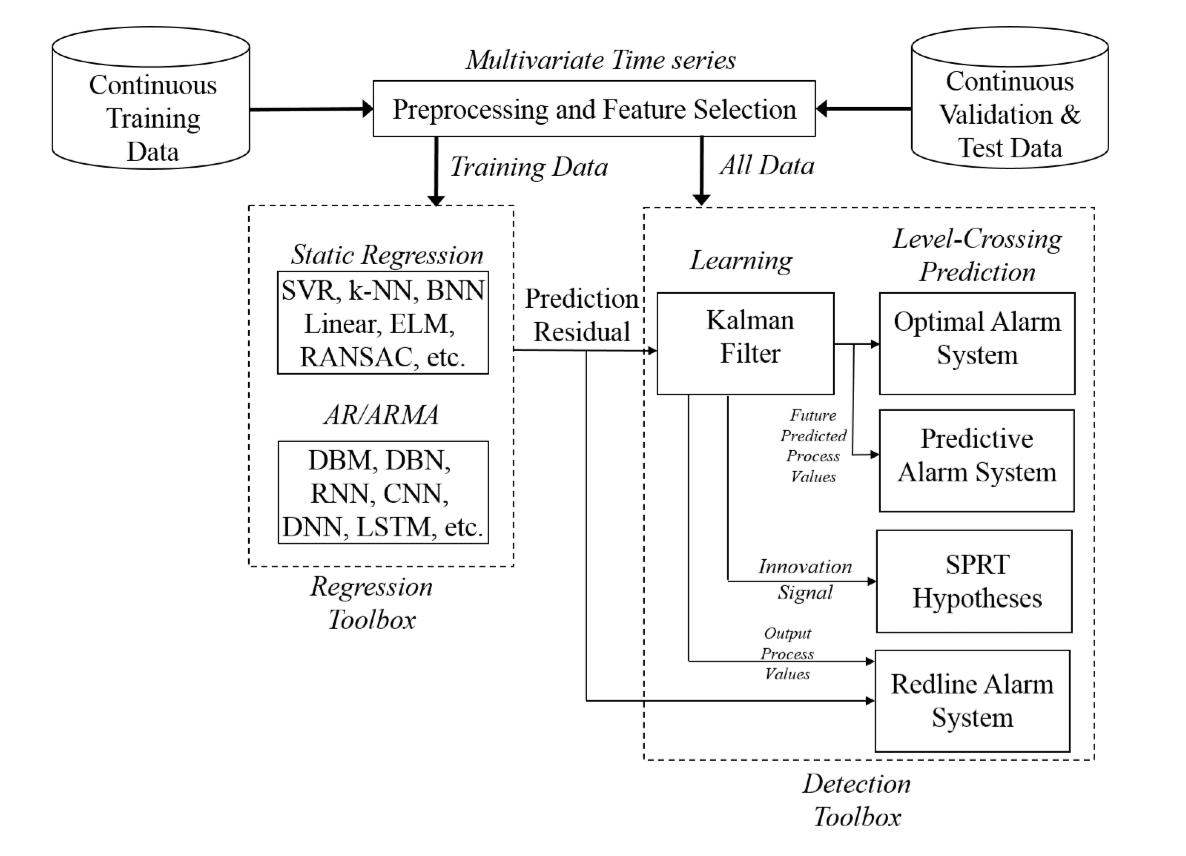
\epsfig{file=figures/arch.png, width=3in}
\caption{ACCEPT Functional Architecture}
\label{fig:accept-arch}
\end{figure}

\subsubsection{Detection Models}
In the detection toolbox, the residuals are used as the basis for learning the underlying linear dynamical system which implicitly models the dynamics that are unable to be captured by the static regression model. Capturing these unmodeled dynamics allows the system to test various statistical hypotheses used by the alarm systems. These unmodeled dynamics are indicated on the signal flow diagram (see Figure \ref{fig:accept-signal}) via the dotted lines.

\begin{figure}[!h]
\centering
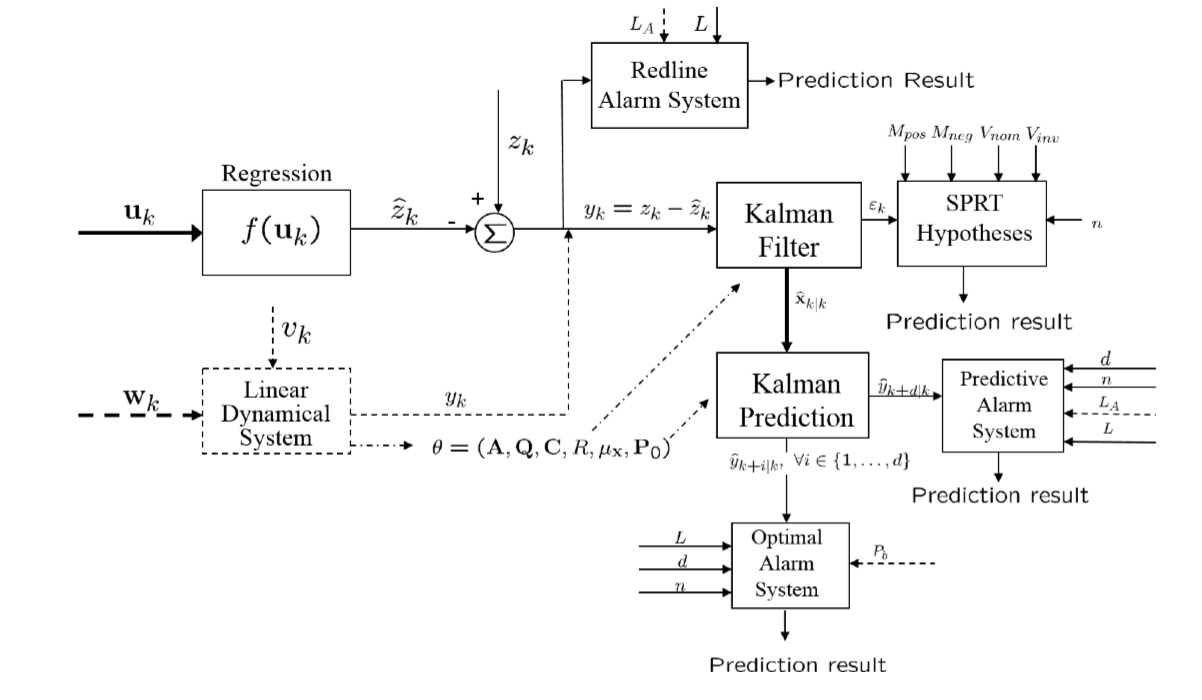
\epsfig{file=figures/signal-flow.png, width=3in}
\caption{ACCEPT Signal Flow Diagram}
\label{fig:accept-signal}
\end{figure}

For the purposes of our project, we are focusing on studying the redline and predictive alarm systems, which use a level-crossing threshold mechanism to initiate an alarm. The difference between the two systems is that the redline alarm system simply uses the current prediction residual values directly as an early warning for prediction of an anomalous event. The predictive alarm system uses future predicted residual values generated from the use of a Kalman Filter in order to determine whether or not an anomalous event will occur in some time horizon. A Kalman Filter predicts future state estimations through Bayesian inference and an estimation of a joint probabilities in each time frame \cite{Kalman}. 

The formal definition for a level-crossing event is given by: \[\mid y_{k+d|k} \mid  > L_a\] where y represents the prediction for d timesteps in advance given the current state k. From Figure \ref{fig:accept-signal}, we can see that the predictive alarm system is supplied several configuration parameters, including the state dimension n and the future prediction horizon d. It is also supplied level-crossing thresholds \begin{math}L, L_a\end{math} which are used to determine the residual value at which an alarm should be generated. These parameters may be chosen based on ROC Curve Analysis, which proceeds in a two-step process. First, the parameters dimension n and horizon d are selected based on maximizing the AUC of the ROC curve generated using the validation data. The second step is finding the ideal threshold(s) via the EER (Equal Error Rate) point, where threshold(s) are selected based on the point where the probability of a false alarm equals the probability of a missed detection, denoted by: \[P_{fa}=P_{md}\] False alarms and missed detections are defined according to the following definition taken from the ACCEPT architecture documentation:

\textbf{False Alarm}: An alarm is triggered at a time point that does not contain an example of a confirmed anomalous event in at least one time point in the next d time steps.

\textbf{Missed Detection}: No alarm is triggered at a time point where an example of a confirmed anomalous event exists in at least one time point in the next d time steps.

The testing data is then used to generate statistics regarding the accuracy of the configured system. For more details on ACCEPT, please refer to \cite{accept}.


\subsection{Cornell University Research \textit{(Victor)}}
Being that we are basing our project off of the NASA ACCEPT framework, we are extending and comparing our results to the work done previously by Brutsaert et al. from Cornell University who used ACCEPT to predict adverse thermal events in NASAs Sustainability Base as well \cite{Cornell}. Because of this, we are attempting to follow in their footsteps with regards to the same values that they input as well as the same targets they optimized for. Our data is primarily the same data that they use, which is out of the possible 2544 sensor variables in the given dataset we are using the same 10 randomly selected features as they are to prevent any possible differences in our results due to training and testing our separate data. In their research, they also fixed a number of target variables such as the detection time as a fixed number of time steps in the future for the detection of adverse events (12 time steps or 1 hour) as well as the targeted temperature that would be considered an adverse event (below 68.1 degrees Fahrenheit). We adopt these constants as well as the dataset that they use.

Their results are also compelling to discuss as they found their best results to be from a Linear Regression model with a Predictive-Training Alarm System, Extreme Learning Machine model with a Predictive-Training Alarm System, and Extreme Learning Machine model with a Predictive-Validation Alarm System. Unlike ACCEPT, our system does not implement the use of training data in the detection phase, therefore all of our results are Validation based. We will go in-depth when we compare our results with theirs, but it is worth noting that surprisingly a model considered to be a relatively simple and basic machine learning method, Linear Regression, did very well in minimizing their False Alarm Rate and Missed Detection Rate.

\section{Regression Toolbox \textit{(Diane/Victor)}}
We begin our discussion of system design by discussing the regression toolbox of our system. This includes preprocessing of the data and various regression models which are compared using cross-validation.

\subsection{Preprocessing \textit{(Diane)}}
Our data collected from different sensors have different ranges. Some fluctuate around 5.0, some fluctuate around 1000.0. In order to improve the accuracy of our model performance and find the precise coefficiency between each feature, we tried to do some preprocessing that mainly focus on standardization.
\subsubsection{Z-score Normalization}
The result of standardization (or Z-score normalization) is that the features will be rescaled so that they'll have the properties of a standard normal distribution \cite{Scaling} with 
\[\mu=0, \sigma=1\]
where $\mu$ is the mean (average) and $\sigma$ is the standard deviation from the mean; standard scores (also called z scores) of the samples are calculated as follows:
\begin{equation} z = \frac{x - \mu}{\sigma}\end{equation}

Standardizing the features so that they are centered around 0 with a standard deviation of 1 is not only important if we are comparing measurements that have different units, but it is also a general requirement for many machine learning algorithms. Intuitively, we can think of gradient descent as a prominent example (an optimization algorithm often used in logistic regression, SVMs, perceptrons, neural networks etc.). With features being on different scales, certain weights may update faster than others since the feature values 
$x_j$ play a role in the weight updates

\begin{equation}\Delta w_j = - \eta \frac{\partial J}{\partial w_j} = \eta \sum_i (t^{(i)} - o^{(i)})x^{(i)}_{j}\end{equation}

\subsubsection{Min-Max Scaling}
An alternative approach to Z-score normalization (or standardization) is the so-called Min-Max scaling (often also simply called ``normalization'' - a common cause for ambiguities).
In this approach, the data is scaled to a fixed range - usually 0 to 1.
The cost of having this bounded range - in contrast to standardization - is that we will end up with smaller standard deviations, which can suppress the effect of outliers.

A Min-Max scaling is typically done via the following equation:
\begin{equation}X_{norm} = \frac{X - X_{min}}{X_{max}-X_{min}}\end{equation}

In the ACCEPT model, it uses z-score scaling to gain better performance. In our research, we tried different standardization methods on different model to get the best performance separately by comparing their lowest median error like min-max standardization for Linear Regression model, z-score for SVM model and none at all in the case of RANSAC. 

\subsection{Regression Algorithm Comparison \textit{(Victor)}}
Just as in ACCEPT the goal of these various regressive models is to model the normal state of the system, thus it is only being run on the training data which does not contain any anomalous events. We partition the training data into several folds for the purpose of k-fold cross-validation analysis and based off of the results select a model minimizing the mean squared error.

In our case, we have considered 6 different regression methods. These being Linear Regression (LR), Extreme Learning Machines (ELM), and Random Sample Consensus (RANSAC), Support Vector Machines (SVM), k-Nearest Neighbors (KNN), and Bagging neural networks (BNN).

Linear Regression, Extreme Learning Machines, and Random Sample Consensus were all selected in order to compare our results to those in the Cornell paper as these three models were the models tested using ACCEPT. However, they each still have unique benefits with regard to possible data inputs.

For Support Vector Machines, k-Nearest Neighbors, and Bagging Neural Networks we discuss their benefits and the reason we selected each model in their respective sections.

\subsubsection{Linear Regression}
Linear regression is a simple forecasting model where through the use of a number of independent variables to fit a line to predict future values\cite{Cornell}.

\subsubsection{Extreme Learning Machine}
ELMs have a structure similar to those of single layer feedforward neural networks but the input layer parameters are assigned randomly. They are special in that training them takes approximately as long as a linear model but also have good generalization performance\cite{Cornell}.

\subsubsection{Random Sample Consensus}
RANSAC is an iterative method that accounts for cases in which the assumptions of typical regression methods do not hold. It is a robust regression method against gross errors and extreme outliers in the data \cite{Cornell}.

\subsubsection{Support Vector Machine}
Support Vector Machines are a set of supervised learning methods, among which include those for regression. They work ideally under circumstances with high dimensional spaces and is memory efficient in its use of a subset of training points in the decision function \cite{svm}. This was selected in part due to the dimensionality of our dataset as we trained based off of 11 different variables but can easily be extended to include more of the over 2000 other variables that Cornell did not use. 

\subsubsection{k-Nearest Neighbors}
k-Nearest Neighbors is a local method that samples nearby cases and predicts a target based off of a similarity measure. This works best for data that is relatively non-volatile and based off of our initial survey of the temperature data this regressive model is applicable.

\subsubsection{Bagging Neural Networks}
Bagging or bootstrap aggregating is an ensemble meta-algorithm designed to improve the stability and accuracy of "unstable procedures" such as neural networks \cite{Breiman96baggingpredictors}. In practicality, this algorithm performs an internal generalization error estimate during its work which is similar to cross-validation, increasing computation time but also reduces variance and helps to avoid overfitting.

\newpage
\section{Detection Toolbox \textit{(Jenna/Federico)}}
In the following sections we discuss the design of our detection toolbox, of which the goal is to create an optimal configuration of a time series modeling process and alarm system to detect future anomalous events in real time. First we will discuss the design of our system, including how residual values from the regression toolbox are used to generate alarms representing anomalous events at some time t. Next, we will discuss the various time-series modeling algorithms used to generate future predictions.

\subsection{Design \textit{(Jenna)}}

In the previous section, we discussed the regression toolbox, which is used to find the best-fitting regression model to fit ideal training data, which contains no anomalous events. For our test dataset, this model will be used to predict future temperature values based on sensor data over time. The purpose of the detection toolbox, is to create a prediction model for the hidden dynamics of the system that the regression model cannot detect. By observing the temperature predictions over time, and measuring the difference between the actual values of the temperatures, we can generate a residual data signal that can be used to predict anomalous events (see Figure \ref{fig:RegressionSignal}). As was previously discussed in the ACCEPT architecture \cite{accept}, the residual data signal can be tested directly to create what is known as a redline alarm detection system, or past residuals can be used to predict future residual values to detect anomalous events. This second kind of system was defined as a predictive alarm system, and has shown to be significantly more effective than the simple redline alarm system for predicting future anomalous events in our data \cite{Cornell}. Our system is modeled after this second kind of system, but unlike ACCEPT we chose to use a variety of time-series modeling algorithms and configurations, to find the best one to suit the data, as opposed to the Kalman filtering system they use. This was done for a variety of reasons, namely that a pure Kalman filter \cite{Kalman} requires knowledge of the state transition model and other parameters, and for that reason can be difficult to configure. We chose to use advanced time-series modeling algorithms that are more general purpose instead, allowing us to test a variety of them and their configurations easily to find the right one for our data.  

\begin{figure}[!h]
\centering
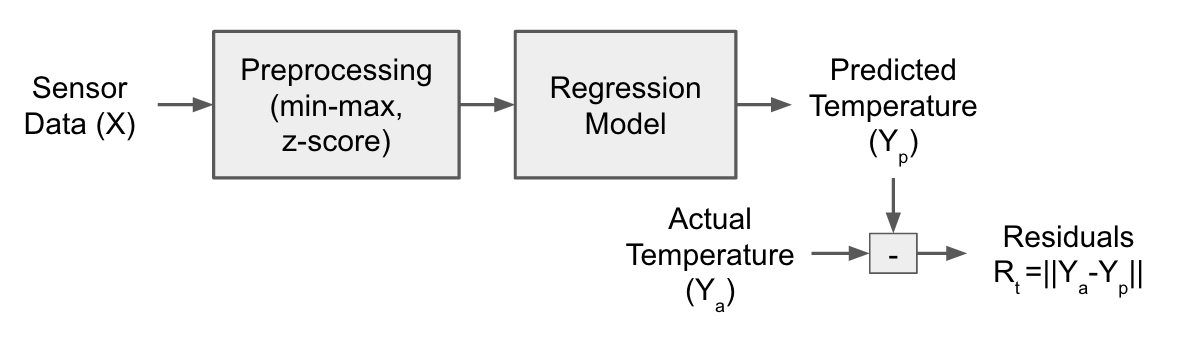
\epsfig{file=figures/regression-signal.png, width=3in}
\caption{Regression Toolbox Signal Flow}
\label{fig:RegressionSignal}
\end{figure}

\subsubsection{Signal Flow}
Figure \ref{fig:DetectionSignal} shows the signal flow diagram for the detection toolbox. At a given time t, past residual data of some length D is used to train the time series model to predict future residual values up to N steps in the future. These future residual values are provided to the predictive alarm system. The predictive alarm system uses the prediction at time t+N in a level crossing mechanism, given by the equation below: \[R_{t+N} > L_a\]    Where \begin{math}L_a\end{math} is an arbitrary threshold value. In order to find the optimal parameters for D, N, \begin{math}L_a\end{math} as well as the optimal time series model to use, the detection process proceeds as follows: First, various D, N and time series model combinations are tested, by generating an ROC curve using the spectrum of possible threshold values. The best models are selected based on their AUC  (Area Under the Curve) for the ROC curve graph (see Figure \ref{fig:rocexample}). This is due to the fact that ROC AUC values are commonly used to predict the probability that a classifier will have a lower chance of error for a randomly chosen value from that curve, however they have been shown to be noisy metric \cite{roc-research}. The second step is taking the top models chosen and selecting a threshold for each based on EER (equal error rate). Errors are defined in a similar fashion to those of ACCEPT, wherein output classification is judged based on the ability to detect an anomalous event in the next N timesteps. Detection error tradeoff information is used to generate a DET (Detection Error Tradeoff) curve, and from that curve the threshold is selected that satisfied the criteria of \begin{math}Pfa = Pmd\end{math} (see Figure \ref{fig:detexample}). The idea behind this step is to find the threshold that minimizes the total error of the system, therefore locating the point that minimizes both values at the same time. At this step, each of the models selected will be completely configured. Throughout this entire process, a set of validation data is used which contains anomalous events, unlike training data, to provide a more accurate fit to the real-world system. Finally, to test the system results are generated using the selected regression algorithm and configuration on the testing data to determine the accuracy of the system.

\begin{figure}[!h]
\centering
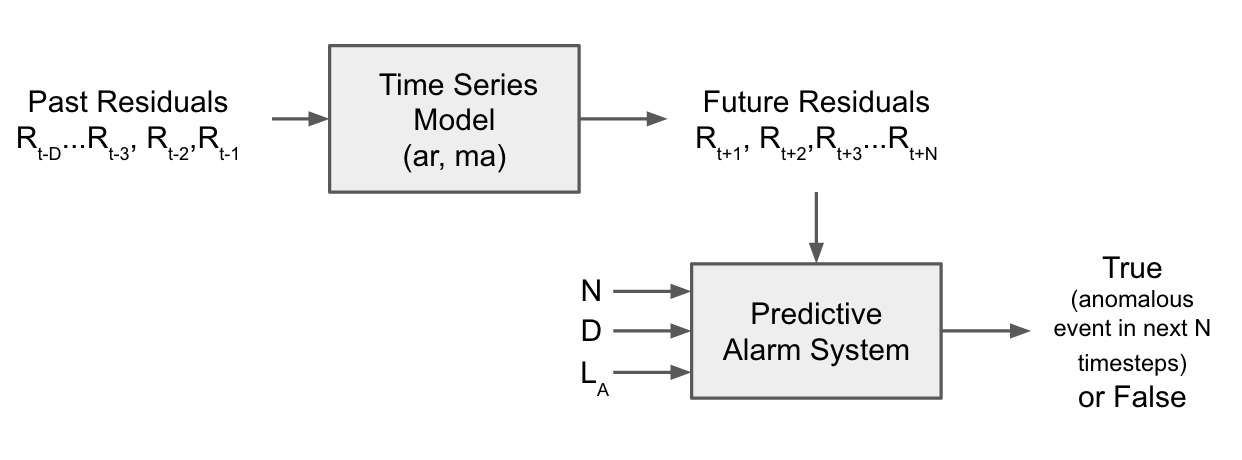
\epsfig{file=figures/detection-signal.png, width=3in}
\caption{Detection Toolbox Signal Flow}
\label{fig:DetectionSignal}
\end{figure}

\subsubsection{Comparison to ACCEPT}
As previously mentioned, our system was modeled after ACCEPT, but differs in the expansion to test various time-series generating algorithms and configurations instead of using a Kalman filtering mechanism. This includes the ability to configure a specific past prediction horizon instead of state space dimension. We also only have fully implemented a predictive alarm system mechanism, instead of a variety of alarm techniques, due to its promising accuracy in prior research \cite{Cornell}. We were also more coarse-grained in our search for correct configuration values, for instance we only used possible past prediction horizons of [16, 32, 48, 64, 80, 96] instead of the full spectrum of possible past horizons. We used methods like this which reduced the accuracy of our system, but allowed us to compute different model combinations in a reasonable amount of time (less than 24 hours) based on our empirical observations about the best data points to test. 

%Added by Federico
\newpage
\subsection{Time-Series Modeling Algorithms \textit{(Federico)}}
The following are the various time series modeling algorithms used within our system.

\subsubsection{ARIMA}

Autoregressive moving average (ARMA) model is based
on a combination of two processes, AR (autoregressive)
and MA (moving average). The basic idea of an AR(p)
model is that the current value, $x_t$, of a stationary series,
can be explained as a linear function of p past values,
$x_{t-1}, x_{t-2},…, x_{t-p}$, where p determines the number of
steps into the past needed to forecast the current value.
The moving average model of order q, abbreviated as
MA(q), assumes the white noise $w_t$ up to lags q are
combined linearly to form the observed data \cite{Kumar:arma}.

ARIMA resembles an ARMA model except that it is presumed 
that the time series has a steady underlying trend (see moving average). 
The model therefore works with the differences between the successive observed values, 
instead of the values themselves. To retrieve the original 
data from the differences requires a form of integration 
and the model is therefore called an autoregressive 
integrated moving average mode \cite{Graham:arima}.

\subsubsection{ARIMAX}

In addition to past values of the response series and past errors, 
one can also model the response series using the current and past 
values of other series, called input series. The ARIMA model with
 input series, also called the ARIMAX model\cite{HYP:HYP9381}.

\subsubsection{GARCH}


Besides modeling the mean process using common
ARIMA time series models, popularized by Box and Jenkins \cite{Box:box}, it appears 
appropriate to incorporate non-linearities and fat-tailed distributions into volatility
modeling.\cite{Zeitlberger2016}

Autoregressive conditionally heteroscedastic (ARCH) models were introduced by Engle \cite{RePEc:ecm:emetrp:v:50:y:1982:i:4:p:987-1007}
and their GARCH (generalized ARCH) extension is due to Bollerslev \cite{RePEc:eee:econom:v:31:y:1986:i:3:p:307-327}. In these models,
the key concept is the conditional variance, that is, the variance conditional on the past. In the
classical GARCH models, the conditional variance is expressed as a linear function of the squared
past values of the series \cite{Francq:garch}.


\subsubsection{Gaussian State Space Models}

State space models are used to represent time-varying systems,
and consist of a latent state process $\{x_t\}_{t=1:T}$ and a related
observation process $\{y_t\}_{t=1:T}$ . The challenge is to infer
the sequence of unknown latent states, and learn parameters of
the model, from the sequence of known observations. It is usually
assumed that the state process is Markovian (i.e., $x_t|x_{t−1}$
is independent of $x_{1:t−2}$ ) and that each observation depends
only on the current state (i.e., $y_t|x_t$ is independent of $x_{1:t−1}$ and
$x_{t+1:T}$ ) \cite{7468569}. 

A basic linear state space model therefore obeys the following
recursive system equations,

\begin{equation}
x_t = Fx_{t-1} + \epsilon_t^x
\end{equation}
\begin{equation}
y_t = Hx_t + \epsilon_t^y
\end{equation}

where $x_t \in \mathbb{R}^{d_x}$ ,$y \in \mathbb{R}^{d_y}$ . $F \in \mathbb{R}^{d_x \times d_x}$ and $H \in \mathbb{R}^{d_y \times d_x}$ are
the transition and observation matrices. $\epsilon_t^x \in \mathbb{R}^{d_x}$ and $\epsilon_t^y \in \mathbb{R}^{d_y}$ 
are the state disturbance and observation noise variables and
we additionally assume that these are drawn from a Gaussian
distribution,

\begin{equation}
\epsilon_t^x \sim \mathcal{N}(0, Q)
\end{equation}
\begin{equation}
\epsilon_t^y \sim \mathcal{N}(0, R)
\end{equation}

where $Q$ and $R$ are positive definite covariance matrices. This
model can be written equivalently in terms of transition and
observation densities,

\begin{equation}
p(x_t|x_{t−1},F,Q)= \mathcal{N}(x_t|Fx_{t−1} ,Q)
\end{equation}
\begin{equation}
p(y_t|x_{t−1},H,R)= \mathcal{N}(y_t|Hx_{t−1} ,R)
\end{equation}


The initial state $x_1$ may be known or may be assigned a Gaussian prior.


\subsubsection{Vovk's Aggregating Algorithm}

The Aggregating Algorithm (AA) \cite{INSR:INSR213} is a general approach
to online learning that involves combining or 'merging' advice
from a pool of experts (typically finite). The objective is to
minimize the losses from a sequence of decisions that must be
made in a stochastic environment. The convergence of the AA is
moderated with a learning rate parameter that can be adjusted for
each particular application but is otherwise constant. The Weak
Aggregating Algorithm (WAA) is similar to the AA but uses a
learning rate parameter that is proportional to $\sqrt{n}$ \cite{Levina2010516}.

% removed \textit{(Federico, everything except regression toolbox)}, too wordy, just put your name on each section individually
\section{Results \textit{(Federico/Victor/Jenna)}}
In this section we present the results of our experiments, using the Sustainable Building public data set \cite{sbdata}. This data set is composed of over 2544 different variables, of which we are utilizing data from 10 of them as predictors, and another sensor, "Building 232 Zone N240 room temperature," as our response variable \cite{Cornell}. The output variable we are observing is a temperature sensor representing the temperature of the primary room experiencing cold events (see Figures \ref{fig:inputvariables} and \ref{fig:outputvariable}). Our goal in creating these results is to design a real time system capable of accurately predicting cold events, measured through the False Alarm (FA) and Missed Detection (MD) rate observed. To have a metric to determine the accuracy of our results vs. those of ACCEPT, we will be comparing our results to those of the Cornell Researchers who ran the same experiment using the same data \cite{Cornell}.

\begin{figure}[!h]
\centering
    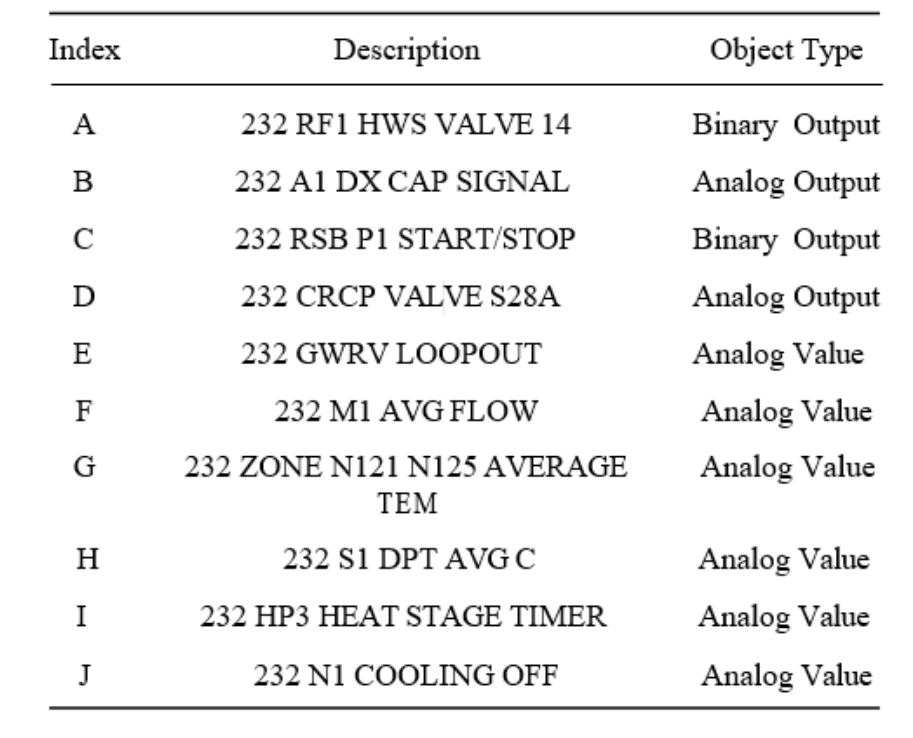
\includegraphics[scale=0.25]{figures/input_variables.png}
\caption{Input variables} 
\label{fig:inputvariables}
\end{figure}

\begin{figure}[!h]
\centering
    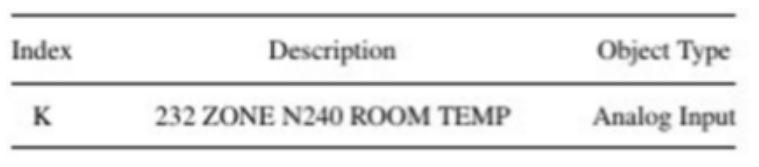
\includegraphics[scale=0.3]{figures/output_variable.png}
\caption{Output variable (Temperature)} 
\label{fig:outputvariable}
\end{figure}

Our complete system is composed of the regression and detection toolboxes, and we will be generating and comparing the results of each in order. Following similar logic as the Cornell University researchers, first an experiment to determine the best regression algorithm was run, including optimal preprocessing of the data. Then a second experiment was made to determine the best detection algorithm. Finally a complete run with the best combination of regression and detection algorithms was done.

\subsection{Regression toolbox results \textit{(Victor)}}
As stated before, six different models were tested, Linear Regression (LR), Extreme Learning Machines (ELM), Random Sample Consensus (RANSAC), Support Vector Machines (SVM), k-Nearest Neighbors (KNN), and Bagging regressor (BNN). We first ran the data through cross-validation without any sort of pre-processing done to the data as shown in Figure \ref{fig:regcomp1}. With this, we found similar results to those found by Cornell in that LR performed the best. It's worth noting that our diagram represents the negative mean squared error on the y axis as opposed to mean squared error, so lower error corresponds to higher positioning on the graph.

After this, we ran the data through various different types of pre-processing to see if the mean squared error could be decreased. We found the lowest median error with SVM, ELM, and LR when using Min-Max scaling, and for KNN and BNN we found the lowest with Z-score normalization. For RANSAC, it was none at all (this is due to the fact that RANSAC itself already performs some probabilistic preprocessing on the data within its run). Using these preprocessing pairings, we ran the algorithms through another 10-fold cross-validation on the training data. Comparing the results in Figure \ref{fig:regcomp2} to the original results in Figure \ref{fig:regcomp1} we can see that preprocessing does indeed slightly improve the results of each regression model, except in the case of SVM where preprocessed training data performed significantly better. SVM was ultimately the best algorithm in this final comparison.

\begin{figure}[!h]
\centering
    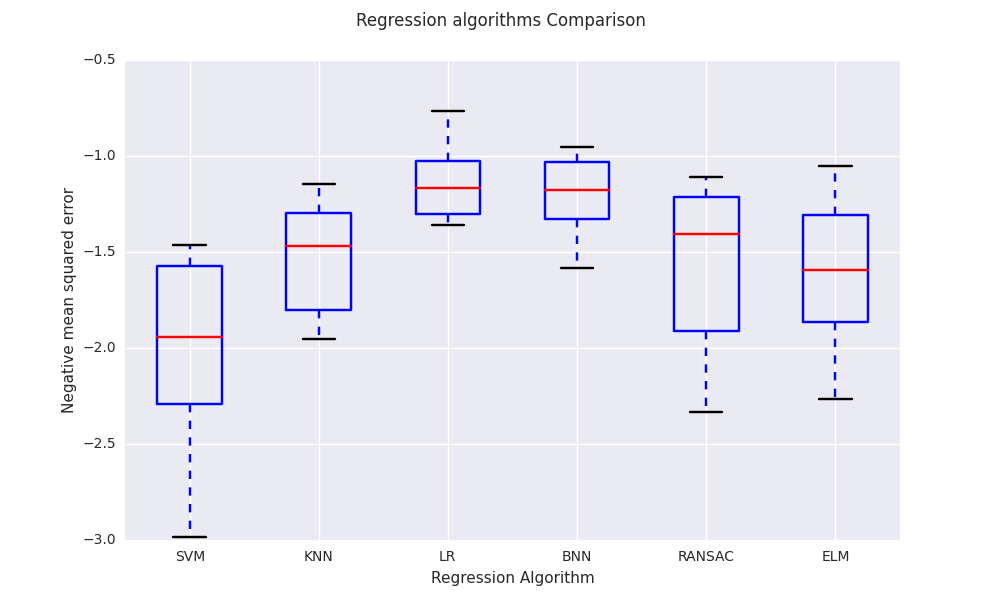
\includegraphics[scale=0.35]{figures/nopre_comparison.png}
\caption{Regression Algorithm Comparison, before Preprocessing} 
\label{fig:regcomp1}
\end{figure}

\begin{figure}[!h]
\centering
    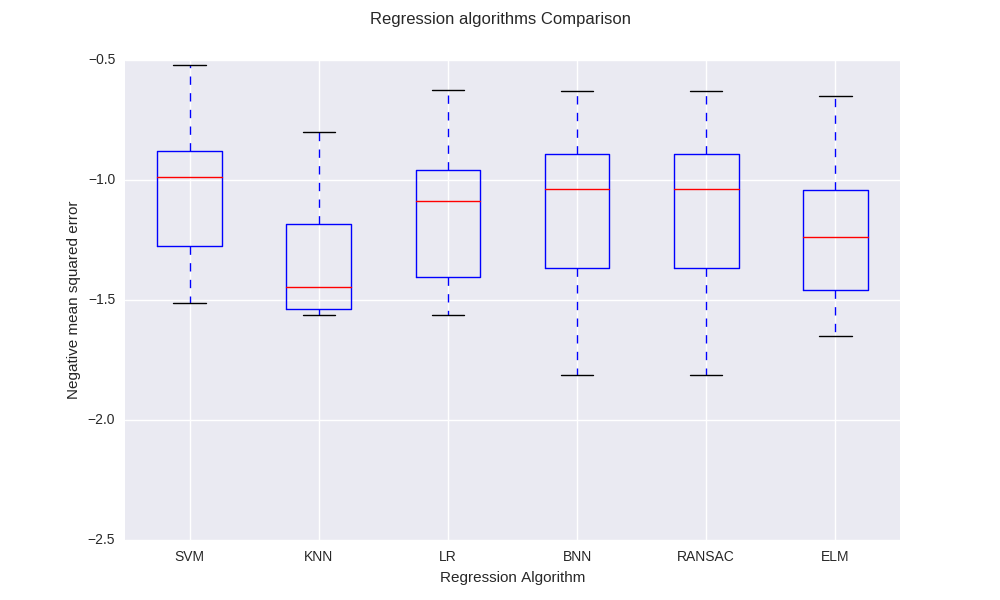
\includegraphics[scale=0.35]{figures/comparision.png}
\caption{Regression Algorithm Comparison, after Preprocessing} 
\label{fig:regcomp2}
\end{figure}


\subsection{Detection Toolbox Results \textit{(Federico/Jenna)}}
% Added/edited by jenna
For choosing the best detection model, many parameters had to be configured in order to compare various time-series models and alarm parameters. As shown in Figure \ref{fig:DetectionSignal}, the detection toolbox takes several parameters, including N, D, and \begin{math}L_a\end{math} for configuring the predictive alarm system, and there are also many different time-series modeling algorithms to choose from. Most of the time-series modeling algorithms take additional parameters, denoted by p and q in the following results. In order to select the best algorithms, empirical observation was used to find a small collection of models and configurations. Since the performance of these models varied when used with various regression models, a variety were ultimately tested.

The following six different algorithm configurations were picked: 
\begin{itemize}
\item ARIMA(p=1, q=1)
\item ARIMA(p=1, q=0)
\item ARIMA(p=2, q=0)
\item ARIMA(p=4, q=0)
\item GARCH(p=1, q=1)
\item Gaussian State Space Model (GGSM)
\end{itemize}

For future consideration of time constraints on a real system, each of these models was compared for time performance. The results of algorithm performance by type can be seen in Table \ref{table:algorithmperformance} located in Appendix B.

Each algorithm was tested with a past prediction horizon in ${32, 48, 64, 80, 96}$. These horizons were also determined empirically, through observation that most models performed most optimally around the middle of this range. The future prediction horizons that were tested include ${6, 12, 18}$.
Our purpose in testing several different future prediction horizons was to observe the relationship between this horizon and the accuracy of the observations. In a real-world system, this parameter may be fixed, depending on the usefulness of receiving an alarm about an impending event in different numbers of future timesteps. Since we are comparing our results to those of the Cornell researchers \cite{Cornell}, we tested the same horizon they chose, of 12 future timesteps which represents one hour of actual time due to the sensor readings being from every 5 minutes. We then chose 6 future timesteps and 18 future timesteps for comparison to shorter or longer horizons, to see if this parameter would have a significant effect on accuracy. Finally, each one of these combinations of the aforementioned models and possible parameters was compared using the
three best regression models from the regression toolbox results: Support Vector Machine, Linear Regression and Bagging Regressor. 

Using these regression models, the residuals over time were computed for the validation data set, which represent the absolute difference between the output of the algorithm and the correct value.

With the predicted residuals, an ROC curve was generated and from it the area under the curve (AUC) value. At the same time,
the ideal threshold was picked based on EER rate. Finally, the algorithms were sorted in by AUC in descending order, with a larger value corresponding to better performance.

The algorithmic representation of this portion of the detection toolbox may be seen in the following pseduocode:

\begin{algorithm}
	\caption{Detection Toolbox Experiment}
	\label{algo:experimenttwo}
	\begin{algorithmic}[1]
    	  \For {$algorithm \in top\_algorithms$}
            \State $AUC\-values = []$
            \For {$model \in time\_series\_models$}
                \For {$past\_horizon \in past\_horizons$}
                    \For {$future\_horizon \in future\_horizon$}
                       \State $AUC\-values.append(compute\-ROC\-AUC(algorithm, model, past\_horizon, future\_horizon))$
					\EndFor 
				\EndFor 
			\EndFor 
			\State $print\ sorted(AUC\-values)$
		\EndFor          
	\end{algorithmic}
\end{algorithm}

The full results from this experiment are shown in figures \ref{fig:svmtop3}, \ref{fig:lrtop3} and \ref{fig:bnntop3} with the data used located in tables \ref{table:svmexperimenttwotop3}, \ref{table:lrexperimenttwotop3} and \ref{table:bnnexperimenttwotop3} of Appendix B.
The results for the top AUC values for each algorithm and prediction horizon have been graphed and grouped by algorithm. Each of the bar colors represents a different future prediction horizon.  As we can see from the graphs, lower future prediction horizon generally corresponds to greater AUC value. We can also see that the performance of the model varies depending on the regression algorithm used to create the residual data over time. All three algorithms overall showed similarities in accuracy when configured using the toolbox settings, but the optimal settings varied for each.
\vspace{.15in}

\begin{figure}[!h]
\centering
    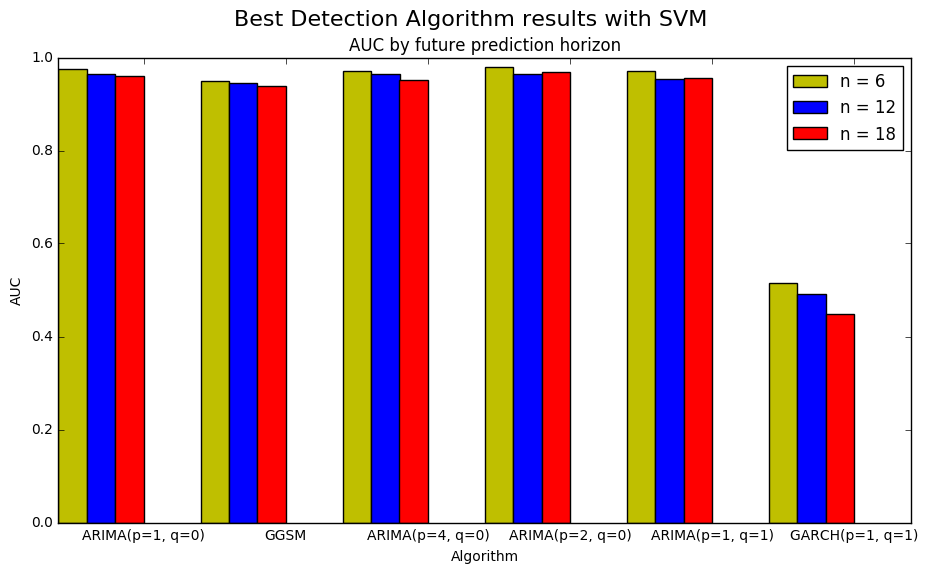
\includegraphics[scale=0.35]{figures/best_detection_svm.png}
\caption{Best Detection Algorithm results with SVM} 
\label{fig:svmtop3}
\end{figure}

\begin{figure}[!h]
\centering
    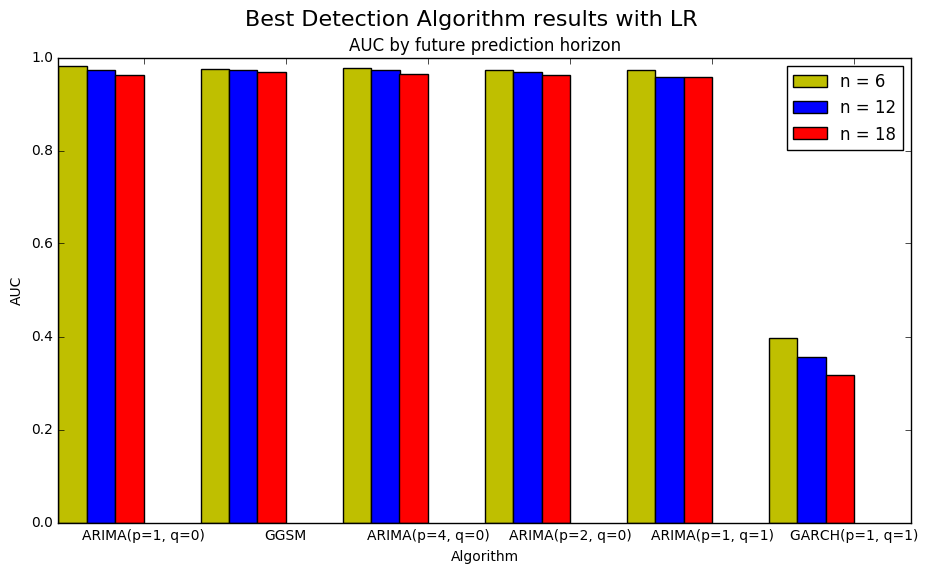
\includegraphics[scale=0.35]{figures/best_detection_lr.png}
\caption{Best Detection Algorithm results with LR} 
\label{fig:lrtop3}
\end{figure}


\begin{figure}[!h]
\centering
    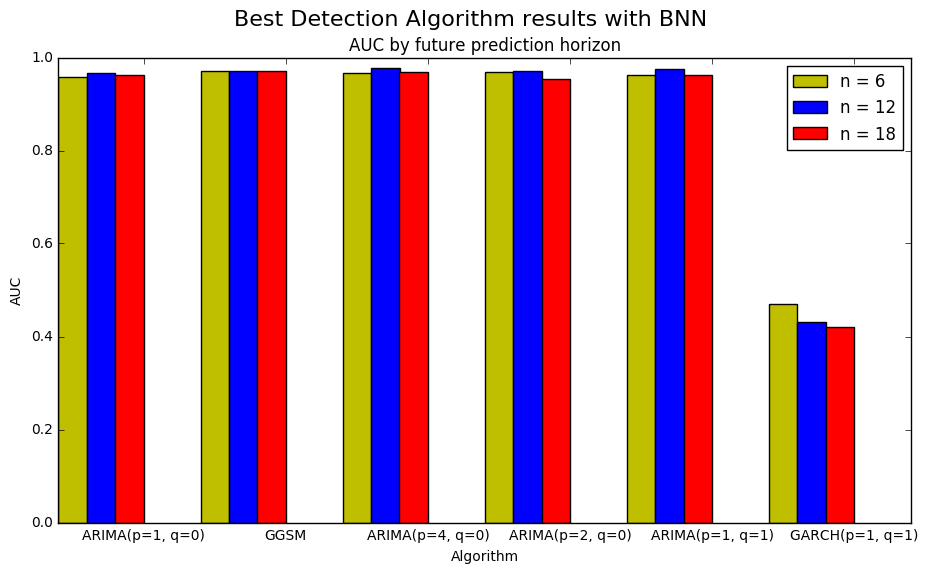
\includegraphics[scale=0.35]{figures/best_detection_bnn.png}
\caption{Best Detection Algorithm results with BNN} 
\label{fig:bnntop3}
\end{figure}

\subsubsection{ROC curve analysis}

Conventionally, the performance of a classification rule is summarized by quantities related to the two types of errors
involved in the decision process: true-positive rate and false-positive rate. The true-positive rate is the probability that a
subject within the studied group is correctly classified within the group (the true-positive rate is also called sensitivity).
The false-positive rate is the probability that a subject outside the group is incorrectly classified within the group (one minus
the false-positive rate is called specificity).

The  receiver operating characteristic is a plot of the true-positive rate (i.e., the ability of the test to detect the characteristic)
 versus the false-positive rate  (i.e., the inability of the test to recognize a normal subject,
without the studied characteristic, as normal) for all possible classification thresholds \cite{Martinez}. 

The area under the ROC curve (AUC) is often used in order to summarize the accuracy of a diagnostic system. In our system
it was used to select the best detection algorithm. An example of an ROC curve generated in our analysis is shown in Figure \ref{fig:rocexample}, with the line of no discrimination shown. The line of no discrimination represents the ROC curve of a completely random classifier, used as the baseline comparison.

\begin{figure}[!h]
\centering
    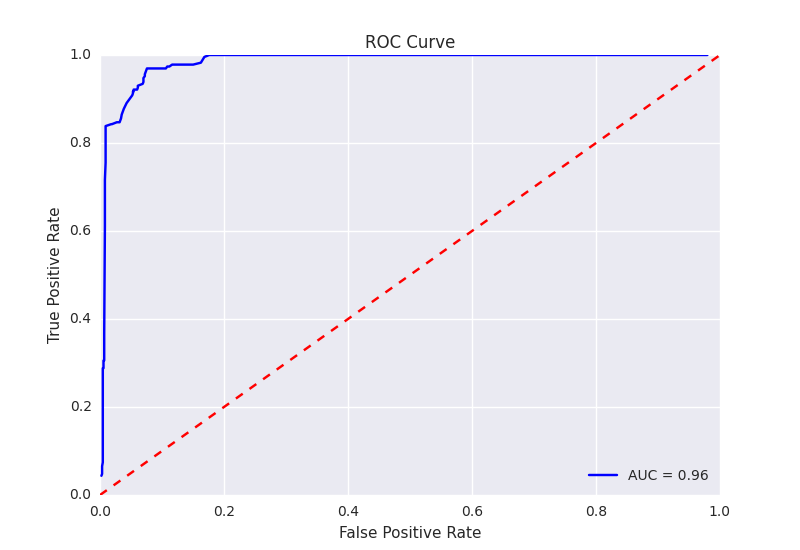
\includegraphics[scale=0.4]{figures/roc.png}
\caption{ROC (Receiver Operating Characteristic) for ARIMA(p=1,q=1), D=32, N=6} 
\label{fig:rocexample}
\end{figure}

\subsubsection{Detection Error Tradeoff}

The false-negative rate or missed-detection rate (MDR), is the probability in a binary classifier that a object is classified as 0 (false)
when the correct value was true. The false-positive rate (FPR), is the opposite case, where the object is classified as 1 (true)
when the correct value was false. If we plot these values over different thresholds, the point, were both are the equal, is called the Equal
Error Rate (EER). We can see in Figure \ref{fig:detexample} and example of a DET graph with the EER selection line given. We use this criteria to select the detection algorithm optimal threshold.


\begin{figure}[!h]
\centering
    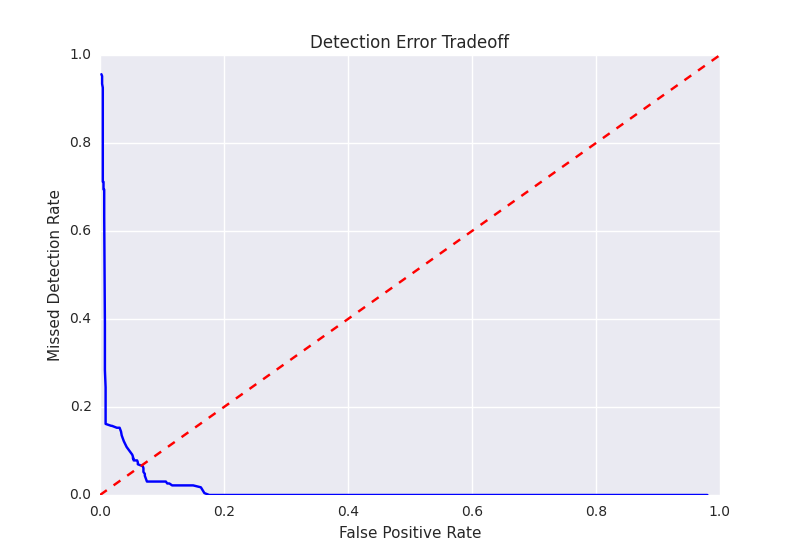
\includegraphics[scale=0.4]{figures/det.png}
\caption{DET (Detection Error Tradeoff) for ARIMA(p=1,q=1), D=32, N=6} 
\label{fig:detexample}
\end{figure}

\subsection{Complete Run Results \textit{(Federico/Jenna)}}

For each combination of regression and detection algorithm tried, the 3 best different algorithms for each future horizon were picked and run with the final testing data. The testing data represents two continuous days from the same time frame, containing anomalous events. The results for this run are shown in figures \ref{fig:svmbest}, \ref{fig:lrbest}, \ref{fig:bnnbest}, of which the data can be found in tables \ref{table:svmbest}, \ref{table:lrbest}, \ref{table:bnnbest} in Appendix B. The performance of the models is shown with the False Alarm Rate (FAR) on the x-axis and the Missed Detection Rate (MDR) on the y-axis. The priority of optimizing for each of these metrics may vary depending on the given application, some systems may require very low MDR or very low FAR. For our application, we assumed that the goal was to minimize the sum of FAR and MDR, to reduce the overall error rate. We analyze our results accordingly, considering results ranked by this sum for performance.




\subsection{Analysis \textit{(Federico/Jenna)}}

Looking at tables \ref{table:svmbest}, \ref{table:lrbest} and \ref{table:bnnbest}, the best result overall was 0.6\% FAR and 3.1\% MDR, and was obtained using BNN, GGSM, past prediction horizon of 64, future prediction horizon of 6 and threshold of 3.225. Its worth  noting there were also favorable results seen for other prediction horizons using the same model. We observed a 0.7\% FAR and a 6.0\% MDR using the same model but with a future prediction horizon of 12. For the future horizon of 18, we observed 0.7\% FAR and 8.8\% MDR. This shows overall strong performance of this model, unlike most of the other models which showed more variance in success at different time horizons.

\subsubsection{Analysis of Time Series Models}
In tables \ref{table:svmexperimenttwotop3}, \ref{table:lrexperimenttwotop3} and \ref{table:bnnexperimenttwotop3}, top results are inversely proportional to the future prediction horizon. This is also true with the testing data.
GARCH was the worst model and in all tests we did it did not generate good results. In contrast all the ARIMA models, in particular the ones with $q=0$, performed really well, same as GGSM. The last one is the most promising  as it does not require parameter optimization. However, as indicated in Table \ref{table:algorithmperformance}, this model also takes the longest to generate, due computing demand required of computing unknown latent states.

Another discovery from these results was that the past prediction horizon needs to be equal or bigger than 48. In addition, all the threshold values discovered were between 2.5 and 4, which give us a rough estimate where the anomaly threshold will be for this dataset.
\vspace{.1in}
\begin{figure}[!h]
\centering
    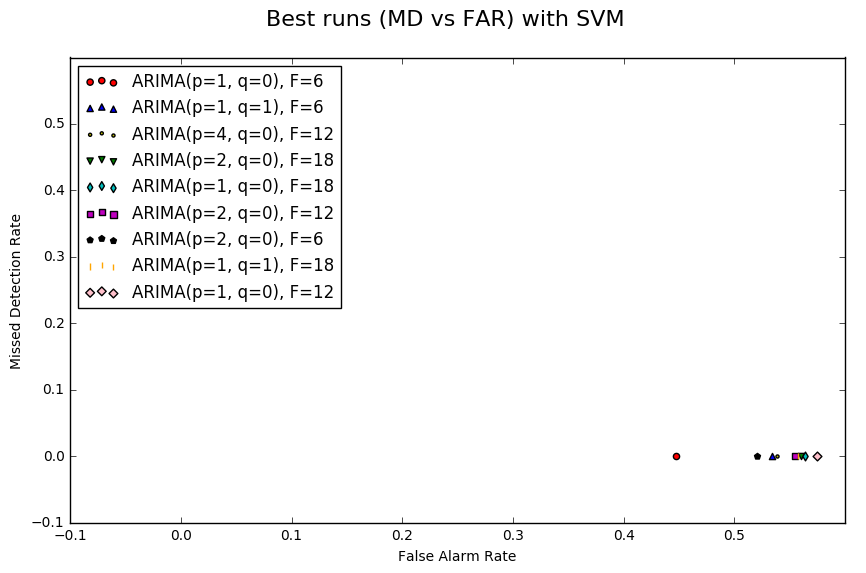
\includegraphics[scale=0.4]{figures/best_runs_svm.png}
\caption{Best Run Results with SVM} 
\label{fig:svmbest}
\end{figure}


\begin{figure}[!h]
\centering
    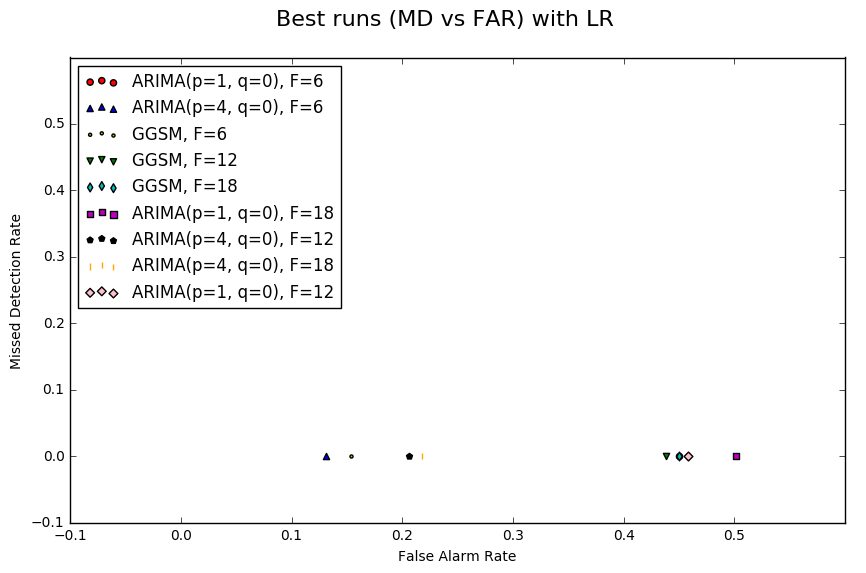
\includegraphics[scale=0.4]{figures/best_runs_lr.png}
\caption{Best Run Results with LR} 
\label{fig:lrbest}
\end{figure}



\begin{figure}[!h]
\centering
    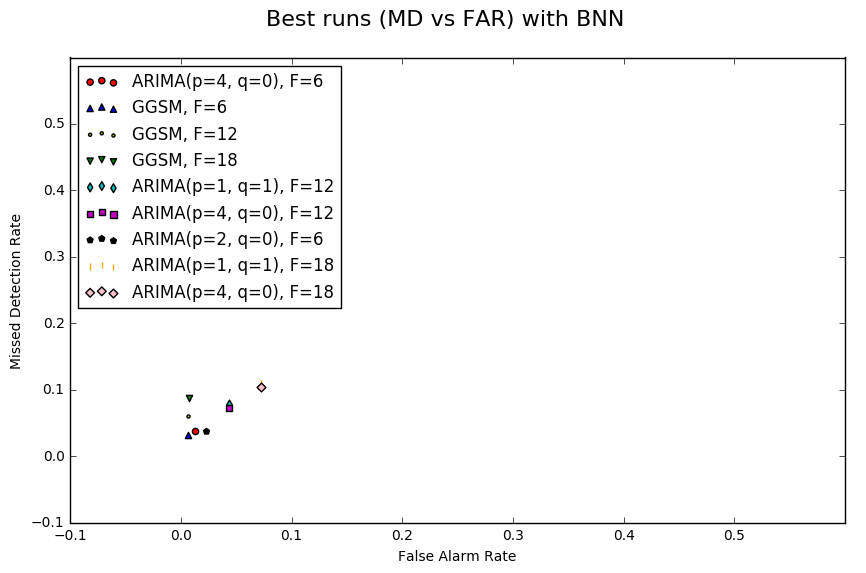
\includegraphics[scale=0.4]{figures/best_runs_bnn.png}
\caption{Best Run Results with BNN} 
\label{fig:bnnbest}
\end{figure}

\begin{table*}[th!]
\centering
\caption{Best Results Overall for Future Horizon of 12}
    \label{table:ourresults}
    \begin{tabular}{|c|c|c|}
        \hline
        Method & False Alarm Rate & Missed Detection Rate \\
        \hline
        \hline
        BNN w/ GGSM & 0.007 & 0.060 \\
        \hline
        BNN w/ ARIMA(p=4, q=0) & 0.043 & 0.072 \\
        \hline
        BNN w/ ARIMA(p=1, q=1) &  0.043 & 0.078 \\
        \hline
    \end{tabular}
\end{table*}


\begin{table*}[th!]
\centering
\caption{Cornell University Results}
    \label{table:cornellresults}
    \begin{tabular}{|c|c|c|}
        \hline
        Method & False Alarm Rate & Missed Detection Rate \\
        \hline
        \hline
        LR w/ Predictive-Training Alarm System & 0.035 & 0.019 \\
        \hline
        ELM w/ Predictive-Validation Alarm System & 0.0138 & 0.0286 \\
        \hline
        ELM w/ Predictive-Training Alarm System & 0.0287 & 0.0333 \\
        \hline
    \end{tabular}
\end{table*}

\vspace{.2in}
\subsubsection{Analysis of Regression Models}
BNN overall had a very strong showing, with all of the top results being under about 10\% for FAR and MDR rates. SVM gave the worst results, followed by LR. Further research needs to be done for SVM as it was the best with the validation data given, but failed to show significant accuracy with the testing data. The results with LR were not surprising due to the simplicity of the model. It is important to notice that SVM and LR both had missed detection rate 0 and high false alarm rate. This is caused because the threshold computed with the validation data is low, thus it does not miss any adverse event, but some of them are false. 

\subsubsection{Time Performance Analysis}
When doing the experiments we also were able to determine the time efficiency each of the algorithm. As there are many factors that can have influence over the design of a system, we created Table \ref{table:algorithmperformance} with a performance approximation that gives an idea on what timing to expect when doing a run with them on this data. As demonstrated by this table, the ARIMA model is the fastest to generate, with only about 3 minutes required to compute the necessary residual predictions on a 2.7 GHz Intel Core i5 machine. GSSM takes the longest, taking approximately 50 minutes to compute the same information. This information may be taken into account when designing a real system, where events may be more frequently generated and computing resources may be limited.


\subsection{Comparison with Prior Research  \textit{(Jenna)}}

Our results rival the ones obtained by Cornell University research team \cite{Cornell}. This may be seen in the summary of their top results in Table \ref{table:cornellresults} and the summary of our top results with the same future prediction horizon in Table \ref{table:ourresults}. We chose to compare based on the same prediction horizon, in order to accurately demonstrate the performance of our system under the same system performance constraint.

We can see that their best results ended up being ELM w/ a Predictive-Validation Alarm system, resulting in false alarm and missed detection rates of 1.38\% and 2.86\%. Our best results came from a BNN-GGSM model with a past prediction horizon of 64, resulting in false alarm and missed detection rates of 0.6\% and 3.1\% respectively. This demonstrates that our system may perform just as well as ACCEPT, for this particular data set. One thing that is curious, is the fact that ELM ended not performing very well in our regression toolbox tests, while ELM ended up being the best performing regression model in the ACCEPT toolbox. This is likely caused by the underlying configuration of the model, in which the defaults were used and no additional configuration was performed to optimize the hyper-parameters of the model. This may have had a significant impact since the number of hidden nodes has a significant impact on ELM performance. Too many nodes can lead to overfitting while too few nodes may lead to underfitting \cite{ELM}. Future work should include a method to configure these hyperparameters in the regression toolbox to further improve the performance of this model.

\section{Conclusion \textit{(Victor)}}
This paper details and constructs an alternative anomaly detection system to that of NASA ACCEPT through the use of open source Python libraries. In modeling ACCEPT, we created a regression toolbox with the help of scikit-learn in order to perform cross-validation and to generate residuals. We then fed these residuals into our detection toolbox which utilized a variety of time series methods from pyflux in order to predict future results and signal alarms. The results that we obtained were not only on par with those generated by Cornell using ACCEPT,they also managed to surpass them in minimizing a number of valued metrics such as Missed Detection Rate and False Alarm Rate. Thus we were successful in our goal of designing a prediction system similar to ACCEPT that is both easier to use and more readily available.

\section{Future Work \textit{(Victor)}}
There are multiple directions that our project could be taken in order to extend and to improve upon multiple aspects of our prediction toolbox.

\subsection{Improving Runtime}
Firstly, an issue that we ran into while working on this project was the runtime of our system. Being written in Python, it ran relatively slowly and could be improved through optimization techniques such as parallelization to multiple threads in order to speed up computation. Due to some of these limitations with regard to computing power, we had to limit the number of models and corresponding parameters we could test in a reasonable amount of time.

\subsection{Improving Results}
The experiments that we ran to find our ideal models were coarse grained and could be made to more finely search through the different values that we varied to tune and improve our models. There were multiple hyperparameters that we did not fully explore. In our regression models, we did not tune any hyperparameters to improve the models to our training cross-validation. For Linear Regression, we used ordinary least squares where we could have used a different version in which we vary regularization coefficients \cite{Cornell}. For our neural network based algorithms such as ELM and BNN, there are a number of hyperparameters that can be tuned, not limited to varying the number of hidden neurons \cite{Cornell}. For ELM specifically, the Cornell results were much better than ours due to this hyperparameter tuning, so it is especially interesting to pursue pruning techniques for the number of hidden neurons such as the Successive Projections Algorithm \cite{ELM}. Then for RANSAC, the cost threshold can be varied to determine the maximum deviation attributable to noise \cite{Cornell}. For kNN, the obvious hyperparameter that can be tuned is k. Then for SVMs, there are two primary parameters that can be varied to improve the model, those being the regularization parameter to minimize training error and model complexity and the Guassian kernel that implicitly defines the nonlinear mapping from input to feature space \cite{Duan03evaluationof}. 

\subsection{Alternate Directions}
Outside of improving our models, there are a number of other things that could be pursued within the scope of this project. There are different parameters that we could optimize for that we could fix while experimenting as to which time series model performs the best under those circumstances, the future prediction horizon specifically is a parameter that can be fixed. While we were attempting to minimize the Equal Error Rate, we could also specifically aim for a certain MDR or FAR while minimizing the other as an example in a real system it may be important to nearly never miss an an alarm making MDR more valuable.

\subsection{Other Projects}
For others interested in using our prediction system, all code is open source and publicly available. Because of this, multiple changes to the code and system are possible. Rather than specifically being applied to temperature and cold events, the code could be changed to accommodate other applications. Further documentation would be important for these goals. See Appendix A for information on accessing, installing and running our software.

%
% The following two commands are all you need in the
% initial runs of your .tex file to
% produce the bibliography for the citations in your paper.
\bibliographystyle{abbrv}
\bibliography{sigproc}  % sigproc.bib is the name of the Bibliography in this case
% You must have a proper ".bib" file
%  and remember to run:
% latex bibtex latex latex
% to resolve all references
%
% ACM needs 'a single self-contained file'!
%
%APPENDICES are optional
%\balancecolumns

\appendix
%Appendix A
\section{Software Guide \textit{(Jenna)}}
In the following section, we describe how to run our project software, hosted online on github at the following link: 

\verb|https://github.com/fedep3/sdl|

\subsection{Software Installation}
Since this project requires the installation of pyflux, matplotlib, scikit-learn and all of their dependencies, we recommend creating a virtual environment on your personal machine and installing all packages there in order to facilitate easy installation. If you are using a Mac OS, you must upgrade your operating system to the latest 2016 version, macOS Sierra, due to Python library dependencies that conflict on older versions of the operating system. Our system requires the installation of Python 2.7, and the following instructions assume it has been installed and is the default version of python installed on your system. 

The following instructions will create a virtual environment and install all dependencies required for our project software in a few easy steps:

Run the following command to install the virtual environment package:

\verb|sudo pip install virtualenvwrapper|

Add the following lines to your .bashrc file:
\begin{verbatim}
export WORKON\_HOME=\$HOME.virtualenvs
export PROJECT\_HOME=/path/to/sdl
source /usr/local/bin/virtualenvwrapper.sh
\end{verbatim}

To create a new virtual environment:
If only Python 2.7 is installed run:
\verb|mkvirtualenv sdl|
Otherwise run:
\begin{verbatim}
mkvirtualenv --python=/path/to/python/2.7 sdl
\end{verbatim}
where \verb|/path/to/python/2.7| represents the path to the python 2.7 executable on your machine

Finally, in order to facilitate easy installation we have listed out package requirements in the requirements.txt file, located in the github. Run the following command to install all packages within the file:

\verb|pip install -r requirements.txt|

Now, each time a terminal is opened and you wish to work on the project, you must run the following command to transition to your new virtual environment: 

\verb|workon sdl|

If one wishes to not use a virtual environment and install the packages globally on a machine, simply run the previous pip command. 

\subsection{Running the Software}

\textbf{Note:} Please refer to the online github link provided to find the most updated version of these instructions.

The software at the time of this writing has 3 modes: regression toolbox mode, detection toolbox mode, and best run mode. The \verb|-t| command line option is used to specify what mode to run, and the optional argument \verb|-r| is used to specify what regression algorithm to use. Use the \verb|-O| python option to suppress debugging output and graph plotting, which is necessary when many different configurations are being run:

\verb|python [-O] main.py [-t type] [-r reg_alg]|

\subsubsection{Regression Toolbox Mode}
To run the regression algorithm comparison and generate the corresponding box plot, use the \verb|-t reg| option, which will run the data preprocessing and regression algorithm comparison and display a box plot representing the statistics on the negative mean squared error for observation.

\subsubsection{Detection Toolbox Mode}
The detection toolbox mode is designed to search for the ideal parameters for a given regression algorithm, and output the best findings ranked by the AUC value. To run this mode, use the \verb|-t det| option, as well as the \verb|-r| option used to specify which regression algorithm to use in the detection toolbox. For instance, to run the detection toolbox using SVM, use the \verb|-r SVM| option.

\subsubsection{Best Run Mode}
This mode is designed to generate final results using testing data. To run it, use the \verb|-t best| option. The best runs are currently hardcoded into this function, including the top results from the top three regression algorithms. The results are ranked based on lowest combined false alarm and missed detection rate.

\section{Full Data Tables}
The following page contains the complete result data tables used to generate the graphs contained within this report.
\balancecolumns
\begin{table*}[h!]
\centering
\caption{Detection Toolbox Top Results with SVM}
    \label{table:svmexperimenttwotop3}
    \begin{tabular}{|c|c|c|c|c|c|c|}
        \hline
        Detection Algorithm & ROC AUC & Past P. H. & Future P. H. & Threshold & False Alarm Rate & Missed Detection Rate \\
        \hline
        \hline
        ARIMA(p=2, q=0) & 0.9786 & 64 & 6 & 2.575 &  0.033 & 0.044 \\
        \hline
        ARIMA(p=1, q=0) & 0.9752 & 48 & 6 & 2.925 &  0.048 & 0.048 \\
        \hline
        ARIMA(p=1, q=1) & 0.9718 & 64 & 6 & 2.575 &  0.041 & 0.044 \\
        \hline
        ARIMA(p=2, q=0) & 0.9690 & 80 & 18 & 2.575 &  0.076 & 0.089 \\
        \hline
        ARIMA(p=2, q=0) & 0.9651 & 80 & 12 & 2.525 &  0.082 & 0.078 \\
        \hline
        ARIMA(p=4, q=0) & 0.9650 & 80 & 12 & 2.575 &  0.064 & 0.070 \\
        \hline
        ARIMA(p=1, q=0) & 0.9642 & 64 & 12 & 2.525 &  0.075 & 0.073 \\
        \hline
        ARIMA(p=1, q=0) & 0.9601 & 80 & 18 & 2.575 &  0.074 & 0.077 \\
        \hline
        ARIMA(p=1, q=1) & 0.9569 & 80 & 18 & 2.575 &  0.083 & 0.085 \\
        \hline
    \end{tabular}
\end{table*}

\begin{table*}[h!]
\centering
\caption{Detection Toolbox Top Results with LR}
    \label{table:lrexperimenttwotop3}
    \begin{tabular}{|c|c|c|c|c|c|c|}
        \hline
        Detection Algorithm & ROC AUC & Past P. H. & Future P. H. & Threshold & False Alarm Rate & Missed Detection Rate \\
        \hline
        \hline
        ARIMA(p=1, q=0) & 0.9808 & 32 & 6 & 3.025 &  0.067 & 0.066 \\
        \hline
        ARIMA(p=4, q=0) & 0.9770 & 48 & 6 & 3.475 &  0.050 & 0.050 \\
        \hline
        GGSM & 0.9763 & 64 & 6 & 3.275 &  0.052 & 0.042 \\
        \hline
        ARIMA(p=1, q=0) & 0.9742 & 48 & 12 & 3.025 &  0.069 & 0.071 \\
        \hline
        GGSM & 0.9729 & 64 & 12 & 3.025 &  0.057 & 0.060 \\
        \hline
        ARIMA(p=4, q=0) & 0.9724 & 48 & 12 & 3.075 &  0.070 & 0.071 \\
        \hline
        GGSM & 0.9698 & 64 & 18 & 2.625 &  0.053 & 0.071 \\
        \hline
        ARIMA(p=4, q=0) & 0.9646 & 64 & 18 & 3.125 &  0.072 & 0.067 \\
        \hline
        ARIMA(p=1, q=0) & 0.9622 & 48 & 18 & 2.975 &  0.081 & 0.078 \\
        \hline
    \end{tabular}
\end{table*}

\begin{table*}[h!]
\centering
\caption{Detection Toolbox Top Results with BNN}
    \label{table:bnnexperimenttwotop3}
    \begin{tabular}{|c|c|c|c|c|c|c|}
        \hline
        Detection Algorithm & ROC AUC & Past P. H. & Future P. H. & Threshold & False Alarm Rate & Missed Detection Rate \\
        \hline
        \hline
        ARIMA(p=4, q=0) & 0.9770 & 96 & 12 & 3.475 &  0.059 & 0.056 \\
        \hline
        ARIMA(p=1, q=1) & 0.9748 & 96 & 12 & 3.275 &  0.069 & 0.068 \\
        \hline
        GGSM & 0.9710 & 64 & 6 & 3.225 &  0.064 & 0.056 \\
        \hline
        GGSM & 0.9701 & 64 & 12 & 3.075 &  0.045 & 0.021 \\
        \hline
        GGSM & 0.9700 & 64 & 18 & 2.925 &  0.029 & 0.028 \\
        \hline
        ARIMA(p=2, q=0) & 0.9694 & 96 & 6 & 3.275 &  0.077 & 0.069 \\
        \hline
        ARIMA(p=4, q=0) & 0.9689 & 96 & 18 & 3.325 &  0.056 & 0.052 \\
        \hline
        ARIMA(p=4, q=0) & 0.9673 & 96 & 6 & 3.425 &  0.065 & 0.074 \\
        \hline
        ARIMA(p=1, q=1) & 0.9621 & 96 & 18 & 3.225 &  0.066 & 0.063 \\
        \hline
    \end{tabular}
\end{table*}

\begin{table*}[h!]
\centering
\caption{Best Run Results with SVM}
    \label{table:svmbest}
    \begin{tabular}{|c|c|c|c|c|c|}
        \hline
        Detection Algorithm & Past P. H. & Future P. H. & Threshold & False Alarm Rate & Missed Detection Rate \\
        \hline
        \hline
        ARIMA(p=1, q=0) & 48 & 6 & 2.925 &  0.447 & 0.000 \\
        \hline
        ARIMA(p=2, q=0) & 64 & 6 & 2.575 &  0.521 & 0.000 \\
        \hline
        ARIMA(p=1, q=1) & 64 & 6 & 2.575 &  0.534 & 0.000 \\
        \hline
        ARIMA(p=4, q=0) & 80 & 12 & 2.575 &  0.538 & 0.000 \\
        \hline
        ARIMA(p=2, q=0) & 80 & 12 & 2.525 &  0.555 & 0.000 \\
        \hline
        ARIMA(p=1, q=1) & 80 & 18 & 2.575 &  0.557 & 0.000 \\
        \hline
        ARIMA(p=2, q=0) & 80 & 18 & 2.575 &  0.561 & 0.000 \\
        \hline
        ARIMA(p=1, q=0) & 80 & 18 & 2.575 &  0.564 & 0.000 \\
        \hline
        ARIMA(p=1, q=0) & 64 & 12 & 2.525 &  0.575 & 0.000 \\
        \hline
    \end{tabular}
\end{table*}

\begin{table*}[h!]
\centering
\caption{Best Run Results with LR}
    \label{table:lrbest}
    \begin{tabular}{|c|c|c|c|c|c|}
        \hline
        Detection Algorithm & Past P. H. & Future P. H. & Threshold & False Alarm Rate & Missed Detection Rate \\
        \hline
        \hline
        ARIMA(p=4, q=0) & 48 & 6 & 3.475 &  0.131 & 0.000 \\
        \hline
        GGSM & 64 & 6 & 3.275 &  0.153 & 0.000 \\
        \hline
        ARIMA(p=4, q=0) & 48 & 12 & 3.075 &  0.206 & 0.000 \\
        \hline
        ARIMA(p=4, q=0) & 64 & 18 & 3.125 &  0.218 & 0.000 \\
        \hline
        GGSM & 64 & 12 & 3.025 &  0.439 & 0.000 \\
        \hline
        ARIMA(p=1, q=0) & 32 & 6 & 3.025 &  0.450 & 0.000 \\
        \hline
        GGSM & 64 & 18 & 2.625 &  0.450 & 0.000 \\
        \hline
        ARIMA(p=1, q=0) & 48 & 12 & 3.025 &  0.458 & 0.000 \\
        \hline
        ARIMA(p=1, q=0) & 48 & 18 & 2.975 &  0.502 & 0.000 \\
        \hline
    \end{tabular}
\end{table*}

\begin{table*}[h!]
\centering
\caption{Best Run Results with BNN}
    \label{table:bnnbest}
    \begin{tabular}{|c|c|c|c|c|c|}
        \hline
        Detection Algorithm & Past P. H. & Future P. H. & Threshold & False Alarm Rate & Missed Detection Rate \\
        \hline
        \hline
        GGSM & 64 & 6 & 3.225 &  0.006 & 0.031 \\
        \hline
        ARIMA(p=4, q=0) & 96 & 6 & 3.425 &  0.013 & 0.037 \\
        \hline
        ARIMA(p=2, q=0) & 96 & 6 & 3.275 &  0.022 & 0.037 \\
        \hline
        GGSM & 64 & 12 & 3.075 &  0.007 & 0.060 \\
        \hline
        GGSM & 64 & 18 & 2.925 &  0.007 & 0.088 \\
        \hline
        ARIMA(p=4, q=0) & 96 & 12 & 3.475 &  0.043 & 0.072 \\
        \hline
        ARIMA(p=1, q=1) & 96 & 12 & 3.275 &  0.043 & 0.078 \\
        \hline
        ARIMA(p=4, q=0) & 96 & 18 & 3.325 &  0.073 & 0.104 \\
        \hline
        ARIMA(p=1, q=1) & 96 & 18 & 3.225 &  0.073 & 0.110 \\
        \hline
    \end{tabular}
\end{table*}

\begin{table*}[h!]
\centering
\caption{Algorithm Time Performance for 2.7 GHz Intel Core i5 Machine}
    \label{table:algorithmperformance}
    \begin{tabular}{|c|c|}
        \hline
        Algorithm & Time Performance \\
        \hline
        \hline
		ARIMA & 3 mins \\
        \hline
		GARCH & 30 mins \\
        \hline
		GSSM & 50 mins \\
        \hline
		Aggregating & > 120 mins \\
        \hline
    \end{tabular}
\end{table*}



% That's all folks!
\end{document}
